%%%%%%%% Group 5 seminar report, ICML 2026 style %%%%%%%%%%%%%%%%%

\documentclass{article}

\usepackage{microtype}
\usepackage{graphicx}
\usepackage{booktabs}

\usepackage{hyperref}

\newcommand{\theHalgorithm}{\arabic{algorithm}}

% Preprint shows author names. The default option hides them and
% prints an ICML review notice, which is the wrong footer here.
\usepackage[preprint]{icml2026}
\makeatletter
\renewcommand{\Notice@String}{LLM Redundancy Seminar, Summer 2026.}
\makeatother

\usepackage{amsmath}
\usepackage{amssymb}
\usepackage{mathtools}

\usepackage[capitalize,noabbrev]{cleveref}

\icmltitlerunning{Neuron-Level Redundancy in Feed-Forward Layers}

\begin{document}

\twocolumn[
  \icmltitle{Neuron-Level Redundancy in Feed-Forward Layers}

  \begin{icmlauthorlist}
    \icmlauthor{Herai Hench}{sem}
    \icmlauthor{Marcel Schlappner}{sem}
    \icmlauthor{Sooraj Rathore}{sem}
    \icmlauthor{Henrik Kunzelmann}{sem}
  \end{icmlauthorlist}

  \icmlaffiliation{sem}{LLM Redundancy Seminar, Technical University of Darmstadt}

  \icmlcorrespondingauthor{Herai Hench}{herai.hench@stud.tu-darmstadt.de}
  \icmlcorrespondingauthor{Marcel Schlappner}{marcel.schlappner@stud.tu-darmstadt.de}
  \icmlcorrespondingauthor{Sooraj Rathore}{sooraj.rathore@stud.tu-darmstadt.de}
  \icmlcorrespondingauthor{Henrik Kunzelmann}{henrik.kunzelmann@stud.tu-darmstadt.de}

  \icmlkeywords{Language Models, Feed-Forward Neurons, Redundancy}

  \vskip 0.3in
]

\printAffiliationsAndNotice{}

\begin{abstract}
Feed-forward layers hold a large share of the parameters in a language model, and it is not obvious which of those units are spare.
We treat a neuron as one channel of the feed-forward activation and mask it with a forward hook, leaving the weights unchanged.
Across GPT-2 (124M--774M), Qwen3-0.6B, Qwen3.5-4B, Qwen3.5-9B, and Llama-2-7B, an importance score equal to activation RMS times the down-projection column norm finds channels whose masking costs less than a random mask of the same size.
Firing rate, layer depth, and model size do not predict that cost in the way we expected.
Near-duplicate neurons are not cheap to delete, but a two-scalar rewrite through the surviving twin recovers the loss in proportion to how well one activation predicts the other.
A short LoRA repairs masking on the smaller models and, at the one budget we could match, overfits at Llama-2-7B.
\end{abstract}

\section{Problem}
\label{sec:problem}

Large language models spend a large share of their parameters in the feed-forward block of each layer.
A natural question is whether some of those units are spare: present in the network, but not doing work that the rest of the model cannot cover.

We studied that at the level of a single neuron.
For us a neuron is one channel of the feed-forward activation, the input to the down-projection.
On a gated model that is one entry of the element-wise product $\mathrm{act}(\mathrm{gate}(x)) \cdot \mathrm{up}(x)$.
On GPT-2 it is one entry of $\mathrm{GELU}(c_{\mathrm{fc}}(x))$.
The channel reaches the residual stream through one column of the down-projection, so its contribution is $h_i \cdot W_{\mathrm{down}}[:, i]$.

We did not remove neurons from the weight matrices.
We masked them with a forward hook, which sets that channel to zero.
Parameter shapes never change, so this report makes no claim about speed, memory, or FLOPs.
Numbers below are relative to each model's own unmasked baseline unless a raw perplexity is given.

\section{Questions}
\label{sec:questions}

We started from a simple plan and had to drop most of it.
\begin{enumerate}
  \item Are some neurons redundant because they rarely fire?
  \item Are middle layers less redundant than early or late layers?
  \item Are larger models more redundant, and does a good ranking pull further ahead of chance as models grow?
  \item Are the neurons that look spare on ordinary text the same ones that look spare on a downstream task?
  \item If two neurons are near-duplicates, is one of them cheap to delete? If not, can its contribution be routed through the other?
  \item After masking, does a short fine-tune undo the damage, and does that get harder as the model gets larger?
\end{enumerate}

\section{Method}
\label{sec:method}

\paragraph{Ranking.}
The score we kept is $\mathrm{RMS}(h_i) \cdot \|W_{\mathrm{down}}[:, i]\|$: how large the activation is, times how strongly that column writes into the residual stream.
This is the same idea as Wanda \citep{sun2024wanda} and LLM-Pruner \citep{ma2023llmpruner}.
We compared it with firing frequency and with a random mask that removes the same number of neurons in each layer.

\paragraph{Masking.}
We zeroed the lowest-scoring neurons at 5\%, 10\%, 25\%, and 50\% of each layer, then measured WikiText-2 perplexity and PIQA accuracy.

\paragraph{Duplicates.}
For pairs with correlation at least 0.9 inside a layer, we masked one twin and compared that with masking an uncorrelated neuron of similar importance.
Separately, we fitted $h_{\mathrm{drop}} \approx \alpha \cdot h_{\mathrm{keep}} + \beta$ on calibration activations and added the dropped twin's contribution back through its partner.
That needs two scalars and no training.

\paragraph{Recovery.}
After importance masking we trained a short LoRA on WikiText-2, and we trained the same adapter on the unmasked model.
The second run is the control.
A LoRA budget can change perplexity even when nothing is masked, which is why the control exists.
On the smaller models that budget helps.
On Qwen3.5-4B and Llama-2-7B the unmasked control got worse.
We report how much of the masking gap remains after both models have had the same budget.

\paragraph{Models.}
GPT-2 at 124M, 355M, and 774M uses GELU and has no gate.
Qwen3-0.6B, Qwen3.5-4B, Qwen3.5-9B, and Llama-2-7B use SwiGLU.
GPT-2 ran in full precision.
The Qwen and Llama runs that did not fit in memory ran in 4-bit.
Qwen3.5-4B was our main model.
The 9B model and the Llama recovery needed a 16\,GB card.

\paragraph{Implementation.}
One calibration pass over WikiText-2 records, per neuron, firing rate, activation size, the importance score above, and pairwise correlation inside a few layers.
A hook on the down-projection applies a mask or, for the duplicate experiment, the fitted replacement.
Evaluation is WikiText-2 perplexity and PIQA.
The same scripts retarget a model by swapping a config file.
Nothing in the intervention changes the parameter tensors.

\section{Findings}
\label{sec:findings}

\subsection{Importance finds spare neurons; firing rate does not}

Importance-ranked masking is cheaper than random masking in every model, and the gap grows as we mask more.
\Cref{fig:masking} shows this on a log scale for six models.
Solid lines with markers are importance, dashed lines are random, and dash-dot lines are firing frequency.
Qwen3.5-9B is not on that plot.
\Cref{fig:9b} is the same comparison for the 9B model alone, and \cref{tab:ppl50} gives the 50\% ratios.
The heading drawn inside \cref{fig:masking} says removal.
The operation is masking.

\begin{figure*}[t]
  \centering
  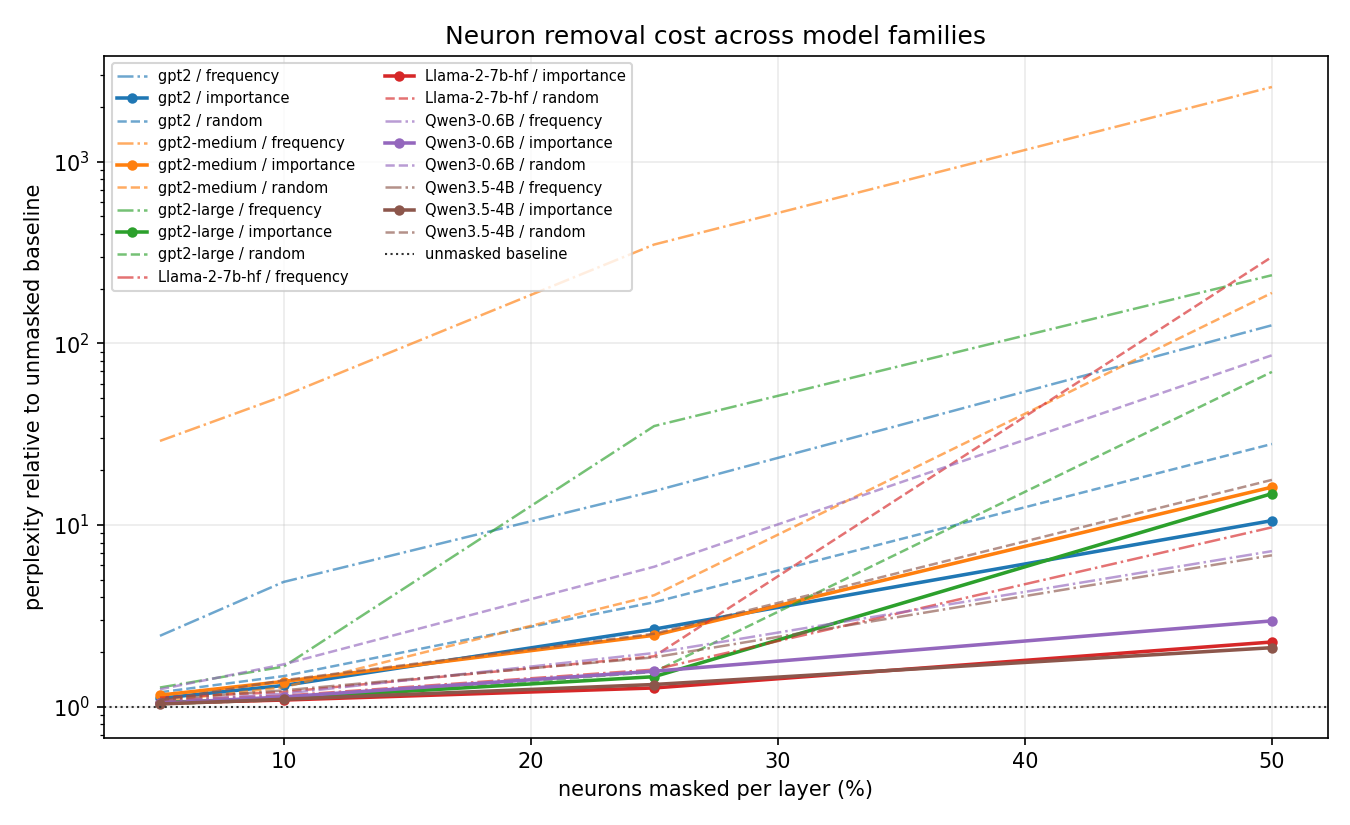
\includegraphics[width=\textwidth,height=0.34\textheight,keepaspectratio]{cross_family_removal.png}
  \caption{WikiText-2 perplexity relative to each model's unmasked baseline, after masking the lowest-scoring feed-forward channels in every layer.
  Solid lines with markers are importance, dashed lines are random, and dash-dot lines are firing frequency.
  Qwen3.5-9B is drawn separately in \cref{fig:9b}.}
  \label{fig:masking}
\end{figure*}

\begin{figure}[t]
  \centering
  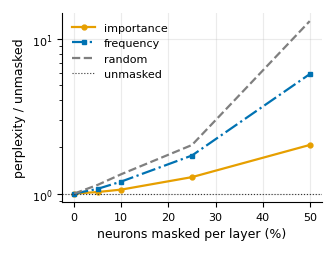
\includegraphics[width=\columnwidth,height=0.28\textheight,keepaspectratio]{qwen35_9b_masking.png}
  \caption{Qwen3.5-9B, shown separately from \cref{fig:masking}.
  WikiText-2 perplexity divided by the unmasked baseline.
  Importance stays near the baseline; frequency sits between importance and random.}
  \label{fig:9b}
\end{figure}

\begin{table}[t]
  \caption{Relative perplexity at 50\% of each layer masked, importance versus random.}
  \label{tab:ppl50}
  \begin{center}
    \begin{small}
      \begin{sc}
        \begin{tabular}{lcc}
          \toprule
          Model & Importance & Random \\
          \midrule
          GPT-2 124M & 10.6$\times$ & 27.9$\times$ \\
          Qwen3-0.6B & 3.0$\times$ & 85.9$\times$ \\
          Qwen3.5-4B & 2.1$\times$ & 17.7$\times$ \\
          Llama-2-7B & 2.3$\times$ & 299$\times$ \\
          Qwen3.5-9B & 2.1$\times$ & 13.0$\times$ \\
          \bottomrule
        \end{tabular}
      \end{sc}
    \end{small}
  \end{center}
  \vskip -0.1in
\end{table}

The ranking transfers across three families and both feed-forward designs.
Llama-2-7B is the clearest case: half the feed-forward channels masked by importance costs about twice the perplexity, and the same count chosen at random costs about 300 times.
PIQA on that model stays at 0.675 against a 0.765 baseline.

Firing frequency was our original plan, following the lazy-neuron phenomenon \citep{li2023lazy}: neurons that rarely fire were expected to be the spare ones.
It is the wrong signal to move across architectures.
On the GPT-2 models it is worse than random at every ratio we tried.
On the gated models it usually beats random and still loses to importance.
GPT-2 is effectively always on, so how often a neuron fires says little about whether it matters.
Two of the gated models (Qwen3.5-4B and 9B) also have almost no silent neurons at our threshold, and frequency still beats random there, so the useful part is the ordering of firing rates, not a pile of dead units.
We did not record that distribution, only the fraction below a cutoff.

\subsection{Depth and size do not behave as expected}

We expected middle layers to be less redundant than early or late layers.
A static summary of importance suggested that.
Masking 10\% of the channels in each depth band and measuring the resulting cost did not confirm this expectation.
\Cref{tab:depth} reports the change in perplexity.
Compare columns within a row.
The baselines differ, so a large change on GPT-2 is not a larger effect than a small change on a 9B model.
\Cref{fig:depth} divides each bar by the worst band in that model, which is what makes the rows comparable.

\begin{table}[t]
  \caption{Change in WikiText-2 perplexity after masking 10\% of the channels in one depth band.
  The bold entry is the most expensive band in that row.}
  \label{tab:depth}
  \begin{center}
    \begin{small}
      \begin{sc}
        \begin{tabular}{lcccc}
          \toprule
          Model & Early & Middle & Deep & Worst \\
          \midrule
          GPT-2 124M & \textbf{+5.24} & +4.08 & +2.31 & early \\
          GPT-2 355M & \textbf{+7.06} & +2.92 & +1.77 & early \\
          GPT-2 774M & +1.06 & +0.98 & +1.01 & flat \\
          Qwen3-0.6B & \textbf{+2.69} & +0.19 & +0.81 & early \\
          Qwen3.5-4B & +0.34 & +0.37 & \textbf{+1.02} & deep \\
          Qwen3.5-9B & +0.16 & +0.14 & \textbf{+0.57} & deep \\
          Llama-2-7B & +0.27 & +0.10 & \textbf{+0.42} & deep \\
          \bottomrule
        \end{tabular}
      \end{sc}
    \end{small}
  \end{center}
  \vskip -0.1in
\end{table}

\begin{figure*}[t]
  \centering
  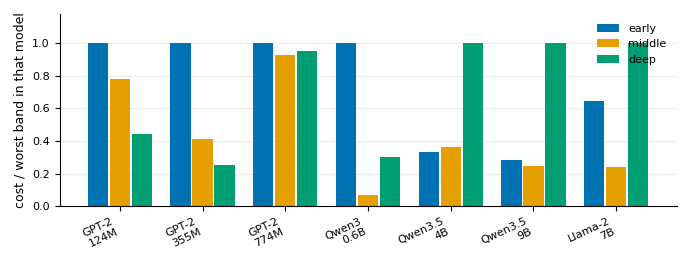
\includegraphics[width=\textwidth,height=0.28\textheight,keepaspectratio]{depth_bands.png}
  \caption{Masking cost by depth band, scaled so the worst band in each model is 1.
  Raw perplexity changes are in \cref{tab:depth}.
  The middle band is never the tallest.}
  \label{fig:depth}
\end{figure*}

The middle band is never the expensive one.
Early layers cost the most on the smaller models.
Deep layers cost the most on the three largest gated models.
The static score ranks neurons inside a layer.
It does not predict what masking a whole band costs.

Size fails in a similar way.
Inside GPT-2, where architecture stays fixed, relative cost at 25\% masking does fall with size (2.67$\times$, 2.47$\times$, 1.46$\times$).
At 10\% and at 50\% it does not, and the static profile barely moves from 124M to 774M.
Inside Qwen the gap between importance and random shrinks as the model grows (3.8$\times$, 1.9$\times$, 1.6$\times$ at 25\%), which is the opposite of what we predicted.
Feed-forward design predicts how well a model tolerates masking better than parameter count does.

\subsection{The task matters on gated models}

We repeated the measurement on PIQA prompts and masked by that ranking instead.
\Cref{tab:task} is at 25\% of each layer.

\begin{table}[t]
  \caption{Each cell is WikiText-2 perplexity / PIQA accuracy at 25\% masking.
  Bold marks the better guided ranking. On GPT-2 that is the WikiText ranking, on both metrics.}
  \label{tab:task}
  \begin{center}
    \begin{footnotesize}
      \begin{sc}
        \begin{tabular}{lccc}
          \toprule
          Model & WikiText & PIQA rank & Random \\
          \midrule
          Llama-2-7B & 12.0 / .750 & 14.3 / \textbf{.785} & 17.9 / .695 \\
          Qwen3.5-4B & 25.0 / .705 & 33.1 / \textbf{.755} & 47.5 / .675 \\
          Qwen3-0.6B & 52.9 / .594 & 94.8 / \textbf{.630} & 199 / .594 \\
          GPT-2 124M & \textbf{138 / .562} & 312 / .544 & 194 / .570 \\
          \bottomrule
        \end{tabular}
      \end{sc}
    \end{footnotesize}
  \end{center}
  \vskip -0.1in
\end{table}

On the gated models, each ranking wins on the data it was fit to.
\Cref{fig:task} is the PIQA half of \cref{tab:task}. The axis starts at 0.50 so the gaps inside a model are visible.
On GPT-2, the PIQA ranking performs worse on both metrics, even compared to random masking for perplexity.
The two corpora still share a core of cheap neurons.
Calibrating on the wrong text costs accuracy.
It does not make the ranking useless.

\begin{figure}[t]
  \centering
  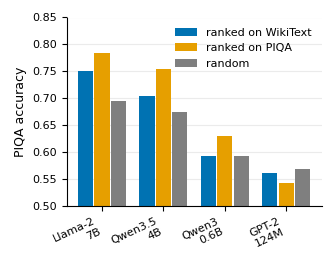
\includegraphics[width=\columnwidth,height=0.28\textheight,keepaspectratio]{task_piqa.png}
  \caption{PIQA accuracy after masking 25\% of each layer.
  On the gated models the PIQA ranking wins.
  On GPT-2 it loses to both the WikiText ranking and to random.
  Perplexity for the same runs is in \cref{tab:task}.}
  \label{fig:task}
\end{figure}

\subsection{Duplicates are cheap to replace, not cheap to delete}

Near-duplicate pairs exist in every model.
Masking one twin of a pair was not reliably cheaper than masking a matched unrelated neuron.
Across seven models the comparison goes one way on three and the other way on four, and wherever the control neuron really matches the twin in importance the difference is a few tenths of a perplexity point or less.

What does work is keeping the information.
When masking a twin degrades performance, routing it through its partner recovers most of the performance loss, with recovery depending on how well one activation predicts the other.
No training is involved.
\Cref{tab:replace} lists the models where masking a twin had a cost.

\begin{table}[t]
  \caption{Replacing a masked twin through its partner.
  Recovered is the share of the masking cost undone by the two-scalar rewrite.}
  \label{tab:replace}
  \begin{center}
    \begin{small}
      \begin{sc}
        \begin{tabular}{lcccc}
          \toprule
          Model & $r^{2}$ & Mask & After & Rec. \\
          \midrule
          GPT-2 124M & 0.90 & +1.16 & $-$0.02 & 102\% \\
          Qwen3-0.6B & 0.89 & +2.24 & +0.28 & 87\% \\
          Llama-2-7B & 0.62 & +0.04 & +0.02 & 47\% \\
          \bottomrule
        \end{tabular}
      \end{sc}
    \end{small}
  \end{center}
  \vskip -0.1in
\end{table}

Correlation says the two neurons move together.
It does not say they have the same scale, so the gain $\alpha$ has to be fitted.
On the models where masking a twin was already free, including Qwen3.5-4B and 9B, there is nothing for replacement to recover, and a percentage there is noise.
Those runs used 22, 14, and 17 pairs on GPT-2 124M, Qwen3-0.6B, and Llama-2-7B.
\Cref{fig:replace} shows the before and after.
On Llama-2-7B both bars are small because masking a twin was already cheap.

\begin{figure}[t]
  \centering
  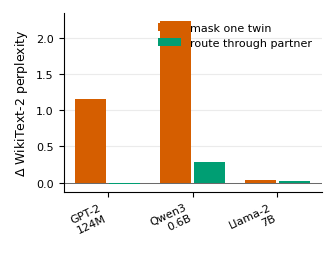
\includegraphics[width=\columnwidth,height=0.26\textheight,keepaspectratio]{replacement.png}
  \caption{Change in WikiText-2 perplexity from masking one twin, and from routing that twin through its partner.
  Qwen3.5-4B and 9B are omitted: masking a twin was already free there, so a recovery percentage is noise.}
  \label{fig:replace}
\end{figure}

\subsection{Short fine-tuning recovers the damage only on the smaller models}

Every recovery run in \cref{tab:lora}, except the 4B row, used the same budget: 200 steps, batch 2, gradient accumulation 4, sequence length 512, about 819 thousand training tokens.
The 4B run used about 51 thousand.

\begin{table}[t]
  \caption{Share of the masking gap closed by LoRA, relative to an unmasked control trained the same way.
  The 4B row used about 51 thousand tokens. Every other row used about 819 thousand.}
  \label{tab:lora}
  \begin{center}
    \begin{small}
      \begin{sc}
        \begin{tabular}{lcc}
          \toprule
          Model & 10\% masked & 25\% masked \\
          \midrule
          GPT-2 124M & 80\% & 87\% \\
          GPT-2 355M & 84\% & 89\% \\
          GPT-2 774M & 76\% & 80\% \\
          Qwen3-0.6B & 76\% & 83\% \\
          Llama-2-7B & \textbf{$-$6\%} & \textbf{48\%} \\
          Qwen3.5-4B & 2\% & --- \\
          \bottomrule
        \end{tabular}
      \end{sc}
    \end{small}
  \end{center}
  \vskip -0.1in
\end{table}

Up through GPT-2 774M and Qwen3-0.6B, most of the masking cost comes back, and model size inside GPT-2 barely matters.
At Llama-2-7B the same budget overfits: training loss falls and WikiText perplexity rises on both the masked model and the unmasked control.
The 4B result looked like the same failure, but that run was not comparable, because it saw 16 times less text.
The 7B run was comparable at 819 thousand tokens, and it still failed.
We did not try a shorter schedule, so this is one training recipe, not a proof that a 7B mask can never be repaired.
Qwen3.5-9B was not fine-tuned.
The 7B run already answers that question at this budget.

\begin{figure}[H]
  \centering
  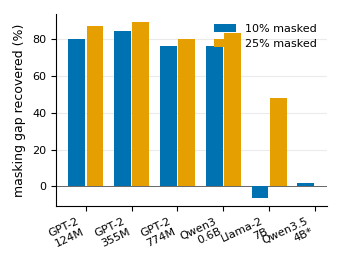
\includegraphics[width=\columnwidth]{lora_recovery.png}
  \caption{Share of the masking gap closed by LoRA, relative to an unmasked control trained the same way.
  Every bar except Qwen3.5-4B* used about 819 thousand tokens.
  That run used about 51 thousand and was not repeated at 25\%.}
  \label{fig:lora}
\end{figure}

\Cref{fig:lora} is the same comparison.
The starred 4B bar is the shorter budget, and it has no 25\% run.

\section{Problems}
\label{sec:problems}

\paragraph{Solved, by changing the method.}
Firing rate saturated on gated models, so we stopped using it as the main ranking.
The depth hypothesis was supported by a static score and rejected by the actual masking experiment, so we stopped treating that score as a substitute for an ablation.
The first duplicate experiment masked the less important twin first, which made the second twin look special for a reason that had nothing to do with duplication.
Replacement compares two treatments of the same neuron and avoids that.

\paragraph{Solved, by more compute.}
The 8\,GB card could not finish a 4-bit Llama-2-7B recovery, because of a library error during evaluation.
We ran the experiment on a 16\,GB GPU.
The same card produced the 9B measurement and masking results.

\paragraph{Still open.}
We never evaluated the image-text model, Qwen3.5-4B, on images.
A neuron that fires only on image tokens would look idle on WikiText and we would call it spare.
Masking is not deletion, so we cannot say the network got faster.
Random baselines are one seed each.
We checked that another seed would not pick a very different amount of importance, but we do not have error bars on perplexity.
The duplicate results rest on a few layers and, in the Qwen3.5 models, on four pairs.
Recovery was tried at one setting.

\section{Conclusion}
\label{sec:conclusion}

Spare feed-forward neurons are real, and an activation-aware score finds them in every model we tested.
How often a neuron fires, which layer it sits in, and how large the model is do not tell you what we thought they would.
A duplicated neuron is not a free deletion.
Its activity is often available in its partner, and a two-scalar rewrite recovers it in proportion to how linear that relationship is.
A short fine-tune repairs masking on the smaller models and, at the budget we could match, overfits at 7B.

\section*{Contributions}

The split below is the work each person is answerable for.
Runs and write-ups were shared as the results came in.

Herai Hench built the experimental pipeline and ran the main 8\,GB campaign: measurement, masking, duplicate-pair tests, replacement, and LoRA recovery, including the GPT-2 size arm that separated model size from architecture.
He also kept the running synthesis of the results into the group reports.

Marcel Schlappner set the measurement and intervention design the later runs followed, and ran the Qwen3.5-4B LoRA recovery on Colab after it did not fit on the shared card.

Sooraj Rathore did the cross-model reading of size and task specificity, and the offline check that the random baselines are not a single unlucky seed.
That pass is what turned several early verdicts into the ones in this report.

Henrik Kunzelmann ran everything that needed a 16\,GB card: the Qwen3.5-9B baseline, then its measurement, masking sweep, depth ablation, and duplicate-pair tests, plus the Llama-2-7B recovery at the same training budget as the smaller models.
Those runs close the size and recovery questions.

\bibliography{references}
\bibliographystyle{icml2026}

\end{document}
